\documentclass[11pt,aspectratio=169,usenames,dvipsnames]{beamer}
\usetheme{SimplePlus}

\usepackage{threeparttable}
\usepackage{booktabs}
\usepackage{xcolor} % For custom colors
\usepackage{tikz} % For styling enumerate numbers
\usepackage{tcolorbox} % For colored box styling
\usepackage{amsmath, amsfonts, amssymb, amsthm} % Math related
\usepackage{natbib}
\usepackage{fontspec}
\usepackage{luatexja}
\usepackage[mathscr]{euscript}

% ---------------- %
% color definition %
% ---------------- %
\definecolor{main}{HTML}{23373B}
\definecolor{pink}{RGB}{180, 50, 110}
\definecolor{orange}{HTML}{FF8000}
\definecolor{red}{HTML}{990000}
\definecolor{blue}{HTML}{004C99}
\definecolor{lightgray}{HTML}{E7E7E7}
\definecolor{gray}{RGB}{90, 90, 90}

\newcommand{\pink}[1]{\textcolor{pink}{#1}}
\newcommand{\orange}[1]{\textcolor{orange}{#1}}
\newcommand{\red}[1]{\textcolor{red}{#1}}
\newcommand{\blue}[1]{\textcolor{blue}{#1}}
\newcommand{\green}[1]{\textcolor{OliveGreen}{#1}}
\newcommand{\magenta}[1]{\textcolor{magenta}{#1}}
\newcommand{\gray}[1]{\textcolor{gray}{#1}}
\newcommand{\purple}[1]{\textcolor{purple}{#1}}
\definecolor{yellow}{HTML}{EDB120}

% \setbeamercolor{alerted text}{fg=blue}

%%% automatically add spaces into enumerate and itemize environment
\let\tempone\itemize
\let\temptwo\enditemize
\renewenvironment{itemize}{\tempone\addtolength{\itemsep}{\fill}}{\temptwo}
\let\tempa\enumerate
\let\tempb\endenumerate
\renewenvironment{enumerate}{\tempa\addtolength{\itemsep}{\fill}}{\tempb}

\usepackage{fontawesome5}
\setbeamertemplate{itemize item}{\faAngleRight}
\setbeamertemplate{itemize subitem}{\faAngleDoubleRight}

\setsansfont{Alegreya Sans Light}[
  ItalicFont={* Italic},
  BoldFont={Alegreya Sans Medium},
  BoldItalicFont={Alegreya Sans Medium Italic}]

\usepackage[mode=tex]{standalone}
\usepackage{tikz}
\usetikzlibrary{decorations}
\usetikzlibrary{decorations.pathreplacing, intersections}
\usepackage{pgfplots}
\usetikzlibrary{calc,positioning}
\usepgfplotslibrary{fillbetween}
\pgfplotsset{compat=newest, scale only axis, width = 10cm}

% --------------------------- %
% Section title page with toc %
% --------------------------- %
\setbeamertemplate{subsection page}{%
    \usebeamertemplate*{section page}
}
\setbeamertemplate{section in toc}[square]
\setbeamertemplate{subsection in toc}[square]
\AtBeginSection[]{
% \sepframe
\begin{frame}[noframenumbering]{Outline}
    % \tableofcontents[currentsection]
    \tableofcontents[currentsection, currentsubsection]
\end{frame}
}
\AtBeginSubsection[]{
  \begin{frame}[noframenumbering]{Outline}
    \tableofcontents[currentsection, currentsubsection]
  \end{frame}
}

% ------------ %
% beamerbutton %
% ------------ %
\newcommand{\goto}[2]{\hyperlink{#2}{\beamergotobutton{#1}}}
\newcommand{\return}[2]{\hyperlink{#2}{\beamerreturnbutton{#1}}}
\newcommand{\extgoto}[2]{\href{#2}{\beamergotobutton{#1}}}

\hypersetup{
    pdfpagemode=UseNone,
    pdftitle = {On ``Reconciling Wage and Price Phillips Curves''},
    pdfauthor = {Hui-Jun Chen},
    pdfsubject = {},
    pdfkeywords = {},
}
\title{On ``Reconciling Wage and Price Phillips Curves''}
\subtitle{by David Osten}
\author{Hui-Jun Chen}
\institute{National Tsing Hua University}
\date{\today}

\begin{document}

% Title Page
\begin{frame}[noframenumbering]
    \titlepage
\end{frame}

\begin{frame}{Overview}
\label{slide:Overview}
\begin{description}[Validate]
    \item[Fact] Price Phillips Curves steepens more than Wage Phillips Curves during tight labor markets
    \vfill
    \item[Data] Document such steepening of PPC comes from market concentration measured by HHI
    \begin{itemize}
        \item Currently pulling data from NFIB for supportive evidence (by Osten)
    \end{itemize}
    \vfill
    \item[Channel] Firms prioritize pricing demand rather than raising wages facing upward wage pressure
    \vfill
    \item[Validate] Most countries (except for four) experiences such channel (NFIB)
    \begin{itemize}
        \item Currently adding MSA analysis (by Osten)
    \end{itemize}
\end{description}
\end{frame}

\begin{frame}{Divergence of PPC and WPC}
\label{slide:Divergence_of_PPC_and_WPC}
    \begin{figure}
        \centering
        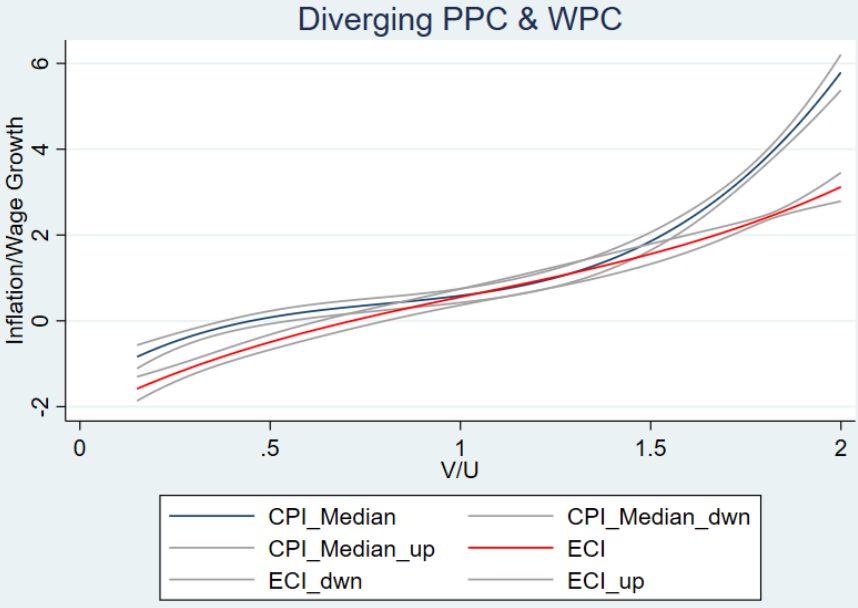
\includegraphics[width=.6\textwidth]{./figures/Fig1.png}
    \end{figure}
\end{frame}


\begin{frame}{Suggestion}
\label{slide:Suggestion}
    % In the writing of introduction,
    % \begin{itemize}
    %     \item I don't think you have defined what is ``UCL'' and ``UCL channel'' in the introduction, and I still don't know what they are after reading the paper. I guess, User cost of labor channel?
    %     \item I think the ``In summary'' paragraph should switch with ``The UCL channel'' paragraph, as ``The UCL channel'' paragraph is talking about mechanism
    % \end{itemize}
    In the connection between model and empirical evidence
    \begin{itemize}
        \item You have provided the evidence on how labor market tightness affects inflation in a highly non-linear fashion.
        \item You have defined the NK-on-the-job-search model in a non-linear fashion as well.
        \item But you derive the PPC and WPC using linear approximation.
        \item \alert{How much of non-linearity do you expect to lose} when you derive model in this way?
    \end{itemize}


\end{frame}


% \appendix

% \begin{frame}[allowframebreaks]{References}
% \footnotesize
% \bibliographystyle{$BIB_STYLE}
% \bibliography{$BIBFILE}
% \end{frame}

\end{document}
